\chapter{Introduction to Project}
The SPIRIT is a very low-power RF transceiver, intended for RF wireless applications in the sub-1 GHz band. It is designed to operate both in the license-free ISM and SRD frequency bands at 169, 315, 433, 868, and 915 MHz, but can also be programmed to operate at other additional frequencies in the 300-348 MHz, 387-470 MHz, and 779-956 MHz bands. The air data rate is programmable from 1 to 500 kbps. 
\section{Overview} 
\noindent SPIRIT2 follows the IEEE802.15.4 protocols. IEEE standard 802.15.4 intends to offer the fundamental lower network layers of a type of wireless personal area network (WPAN) which focuses on low-cost, low-speed ubiquitous communication between devices. It can be contrasted with other approaches, such as Wi-fi, which offer more bandwidth and require more power. The emphasis is on very low cost communication of nearby devices with little to no underlying infrastructure, intending to exploit this to lower power consumption even more. The basic framework conceives a 10-meter communications range with a transfer rate of 250 kbit/s. Tradeoffs are possible to favor more radically embedded devices with even lower power requirements, through the definition of not one, but several physical layers. Lower transfer rates of 20 and 40 kbit/s were initially defined, with the 100 kbit/s rate being added in the current revision. IEEE 802.25.4 includes the lower layer i.e; PHY and MAC layer. 6lowPAN sits on the top of the wpan devices and act as the convergence layer to be used by the normal IPv6 kernel stack. 6LowPAN transparently handles the fragmentation and defragmentation between the different maximum transmission units(MTU’s) (127 vs 1280) as well as compressions.\\
\noindent The host system must be able to communicate with SPIRIT in order to set straight the relationships and interaction between various portions of the stack. These communications are of course handled by the Operating System. Furthermore for the OS to communicate with an external peripheral, device drivers are employed. And this is the whole idea of this project: creating a device driver for SPIRIT so that it can be used in conjunction with systems running on Linux based operating systems.\\
\noindent The device driver ensures that the peripheral is able to communicate with the host but the way this communication is to be conducted depends on what physical connection options are offered by the peripheral. In case of the SPIRIT the physical interface is SPI. Once the means of communication are fixed, there comes the question of deciding which part of the protocol is to reside on which side the host or the peripheral. It will be seen in later chapters as to how the whole stack has been fragmented in this project.\\
\noindent Linux is written in C and so are the device drivers for Linux. 
\section{Existing system}
\noindent WPAN has been a prominent technology in networking and has been the backbone of many user applications. As such it only makes sense that an operating system incorporates enough attention to WPAN as a technology. And this is exactly the case with Linux. It was realized early on that WPAN is going to be a major player and hence efforts were made to have it be an integral part of Linux. The software side of WPAN is official WPAN protocol stack for Linux i.e. linux-wpan which will be looked at in later sections of this report. The other major thing that then remains is the hardware: the SPIRIT. Due to increase in number of interconnect devices these days there is a greater need of software infrastructure to support these devices .Since the underlying hardware is a RF Device, and Linux is the Freely available OS with a large base of community support it is dire necessity to develop a Linux RF driver for the ST’s Sub-Ghz hardware – SPIRIT1 and SPIRIT2.\\
\noindent This is of course possible because Linux, the OS has a stack support for SPI, so once a hardware is detected then all that remains is to bridge this stack to the device using some standard protocol. All of this is taken care by the device driver for that particular device. It is simple, in order for a device to be supported, there has to be a device driver for it, and in this section. I describe some of the widely used WPAN devices that are supported by Linux at the time this writing:\\
like Android, Meego ,Moblin ,RT-Linux and to larger base of Interconnect devices running Linux – Like routers, network hubs, IoT devices and wearables. at86rfxxx, mrf24j40, cc2520.
\subsection{ATMEL at86rf230}
The AT86RF230 is a low-power 2.4 GHz radio transceiver which is developed by the ATMEL. Atmel Corporation is an American-based designer and manufacturer of semiconductors, founded in 1984. The company focuses on embedded systems built around microcontrollers. at86rf230 especially designed for ZigBee/IEEE 802.15.4 applications. The AT86RF230 follows the SPI for the communication with the OS. All RF-critical components except the antenna, crystal and de-coupling capacitors are integrated on-chip. This single-chip radio transceiver provides a complete radio transceiver interface between the antenna and the microcontroller. It comprises the analog radio transceiver and the digital demodulation including time and frequency synchronization, and data buffering. In June 2014 they provide the software support for their device in linux. The low power consumption of the device make it highly popular for the linux OS and after that atmel developed many version of this transceiver(under this series at86rfxx).
\begin{figure}[ht]
	\centering
	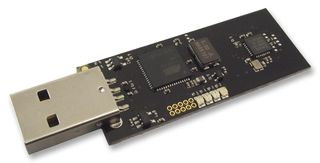
\includegraphics[scale=0.8]{images/atmel.jpg}
	\caption{atmel transceiver}
\end{figure}
\subsection{Microchip mrf24j40}
The MRF24J40 is an IEEE 802.15.4 Standard com­pliant 2.4 GHz RF transceiver. It is the product of Microchip. Microchip Technology is an American manufacturer of microcontroller, memory and analog semiconductors. Its products include microcontrollers (PIC micro, PIC32) Serial EEPROM devices, Serial SRAM devices, radio frequency (RF) devices. It integrates the PHY and MAC functionality in a single chip solution. The MRF24J40 creates a low-cost, low-power, low data rate (250 or 625 kbps) Wireless Personal Area Network (WPAN) device. The MRF24J40 interfaces to many popular Microchip PIC microcontrollers via a 4-wire serial SPI interface, interrupt, wake and Reset pins.\\ 
\noindent The MRF24J40 is compatible with Microchip's ZigBee, MiWi and MiWi P2P software stacks. It works in various mode but the IEEE 802.15.4 feature is supported only in normal mode and each TX FIFO has a specific purpose depending on if the mrf24j40 is configured for beacon and non-beacon-enabled mode. Microchip offers this transceiver in various OS. 
\begin{figure}[ht]
	\centering
	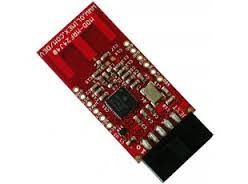
\includegraphics[scale=0.8]{images/microchip.jpg}
	\caption{Microchip transceiver}
\end{figure}
\subsection{Texas CC2520}
The CC2520 is TI's second generation ZigBee IEEE 802.15.4 RF transceiver for the 2.4 GHz unlicensed ISM band. Texas Instruments Inc. (TI) is an American technology company that designs and manufactures semiconductors, which it sells to electronics designers and manufacturers globally headquartered in Dallas, Texas, United States, TI is one of the top ten semiconductor companies worldwide, based on sales volume. This chip enables industrial grade applications by offering state-of-the-art selectivity/co-existence, excellent link budget, operation up to 125°C and low voltage operation. CC2520 has 6 GPIO pins that can be individually configured as inputs, outputs and activate pull-up resistors. There are other solutions by Texas for Wpan as well and they work well with Linux as the driver is there for them.

\begin{figure}[ht]
	\centering
	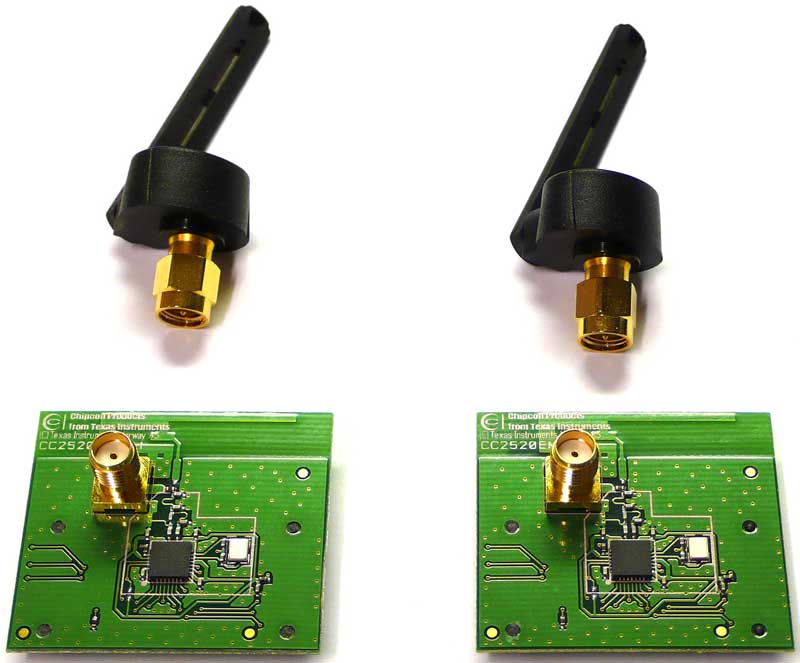
\includegraphics[scale=0.3]{images/texas.jpg}
	\caption{Texas transceiver}
\end{figure}
\section{Requirement Analysis}
There are many wpan adapters out there that have well documented and tested support in Linux based operating systems. Linux being an open source kernel is always inviting people to look into its internal working and stack flow in order to contribute in it.\\
STMicroelectronics excels at grabbing newer opportunities and always be ready with solutions that are on par or even transcends other solutions in the market in a wide range of technologies. The Wpan technology is no different. ST has its fair share of Wpan modules. But thing to be considered here is that even though ST has a wide range of Wpan solutions, none has Linux support.\\ 
So the major requirement of this project was to take a Wpan transceiver by ST and add its support to Linux. And again Linux being open source makes the job much simpler. The module that was considered is the SPIRIT2 transceiver which is SPI based. So the whole requirement of this project can be summed up as adding support (writing a device driver) in Linux (because it is open source and one of the most popular OS kernels in the world) for the Wpan module offered by STMicroelectronic i.e. SPIRIT1 and SPIRIT2.\\
In order to fulfill the above stated requirement it is essential to look into both sides of the coin: Linux driver development and how is the wpan stack being represented there; and then SPIRIT and what portion of the stack is on it and how much of it is needed in order to work with Linux.\\
As SPIRIT2 follows the IEEE 802.1.4 protocols. 802.15.4 covers the lower layer the physical layer and the medium acess control but the good news here is that in linux already there is a support of 802.15.4 so we have to write the driver for our device and then registered that device on the IEEE 802.15.4 platform, for that we have to we have to look into the physical layer i.e. RF layer.\\ 
Another important point to consider is that how the connection is to be made between the Host (running on Linux) and SPIRIT2. SPIRIT2 is based on Serial Peripheral Interface, and in linux already there is the support for Serial peripheral interface so that is exactly what is required to be used for the connections. 
\section{Feasbility Study}
As stated in the requirement analysis section, there are two things that are needed to be considerd here:
\subsection{Does SPIRIT support what wpan offers?}
The answer is yes. Wpan follows the IEEE802.15.4. These are the specification from the IEEE's 802.15 working group, which tackles wireless "personal area" networks, or WPANs. The standard defines a physical-layer and media access control specification, meaning that it covers the frequencies and negotiation options of the connection, but not the protocols that run above it. The communication between between the two spirit is to be held through the 6lowpan these are also the standard developed by the IETF.\\
The 6LoWPAN concept originated from the idea that "the Internet Protocol could and should be applied even to the smallest devices and in linux already there is a support for the 6lowpan because many transceiver from other manufacturer stated early follows the 6lowpan for communications. We will discussed later that how the frame format for transmission of Ipv6 packets as well as well the formation Ipv6 link-local addresses and statelessly auto configured data on the top of IEE802.15.4 networks. Since Ipv6 support of packet size much larger than the largest IEEE802.15.4 frame size, an adaption layer is defined. 
\subsection{Does Linux supports what SPIRIT used to communicate?}
SPIRIT is based on SPI. Any form of communication between the host and SPIRIT is to be had through the Serial Peripheral Interface. There are many SPI based driver in Linux for the wpan.   There are also many network drivers that allow the communication between the host and the controller through SPI. So following the same footsteps it should be possible to send commands from the host to the controller using SPI.\\
Considering the above things, it seems feasible to write a driver for SPIRIT in Linux. The driver shall essentially act as a bridge between SPIRIT protocol stack residing partly in the user space and partly in the kernel space of Linux and SPIRIT.
\section{Objectives of the Project}
\begin{itemize}
	\item To setup a SPIRIT driver interface for SPI.
	\item To make a entry for SPIRIT in sysfs.
	\item To map the IEEE 802.15.4 commands with the SPIRIT2.
	\item To interface the SPI Commands from SPIRIT to host.
\end{itemize}
